\subsubsection{Bind}

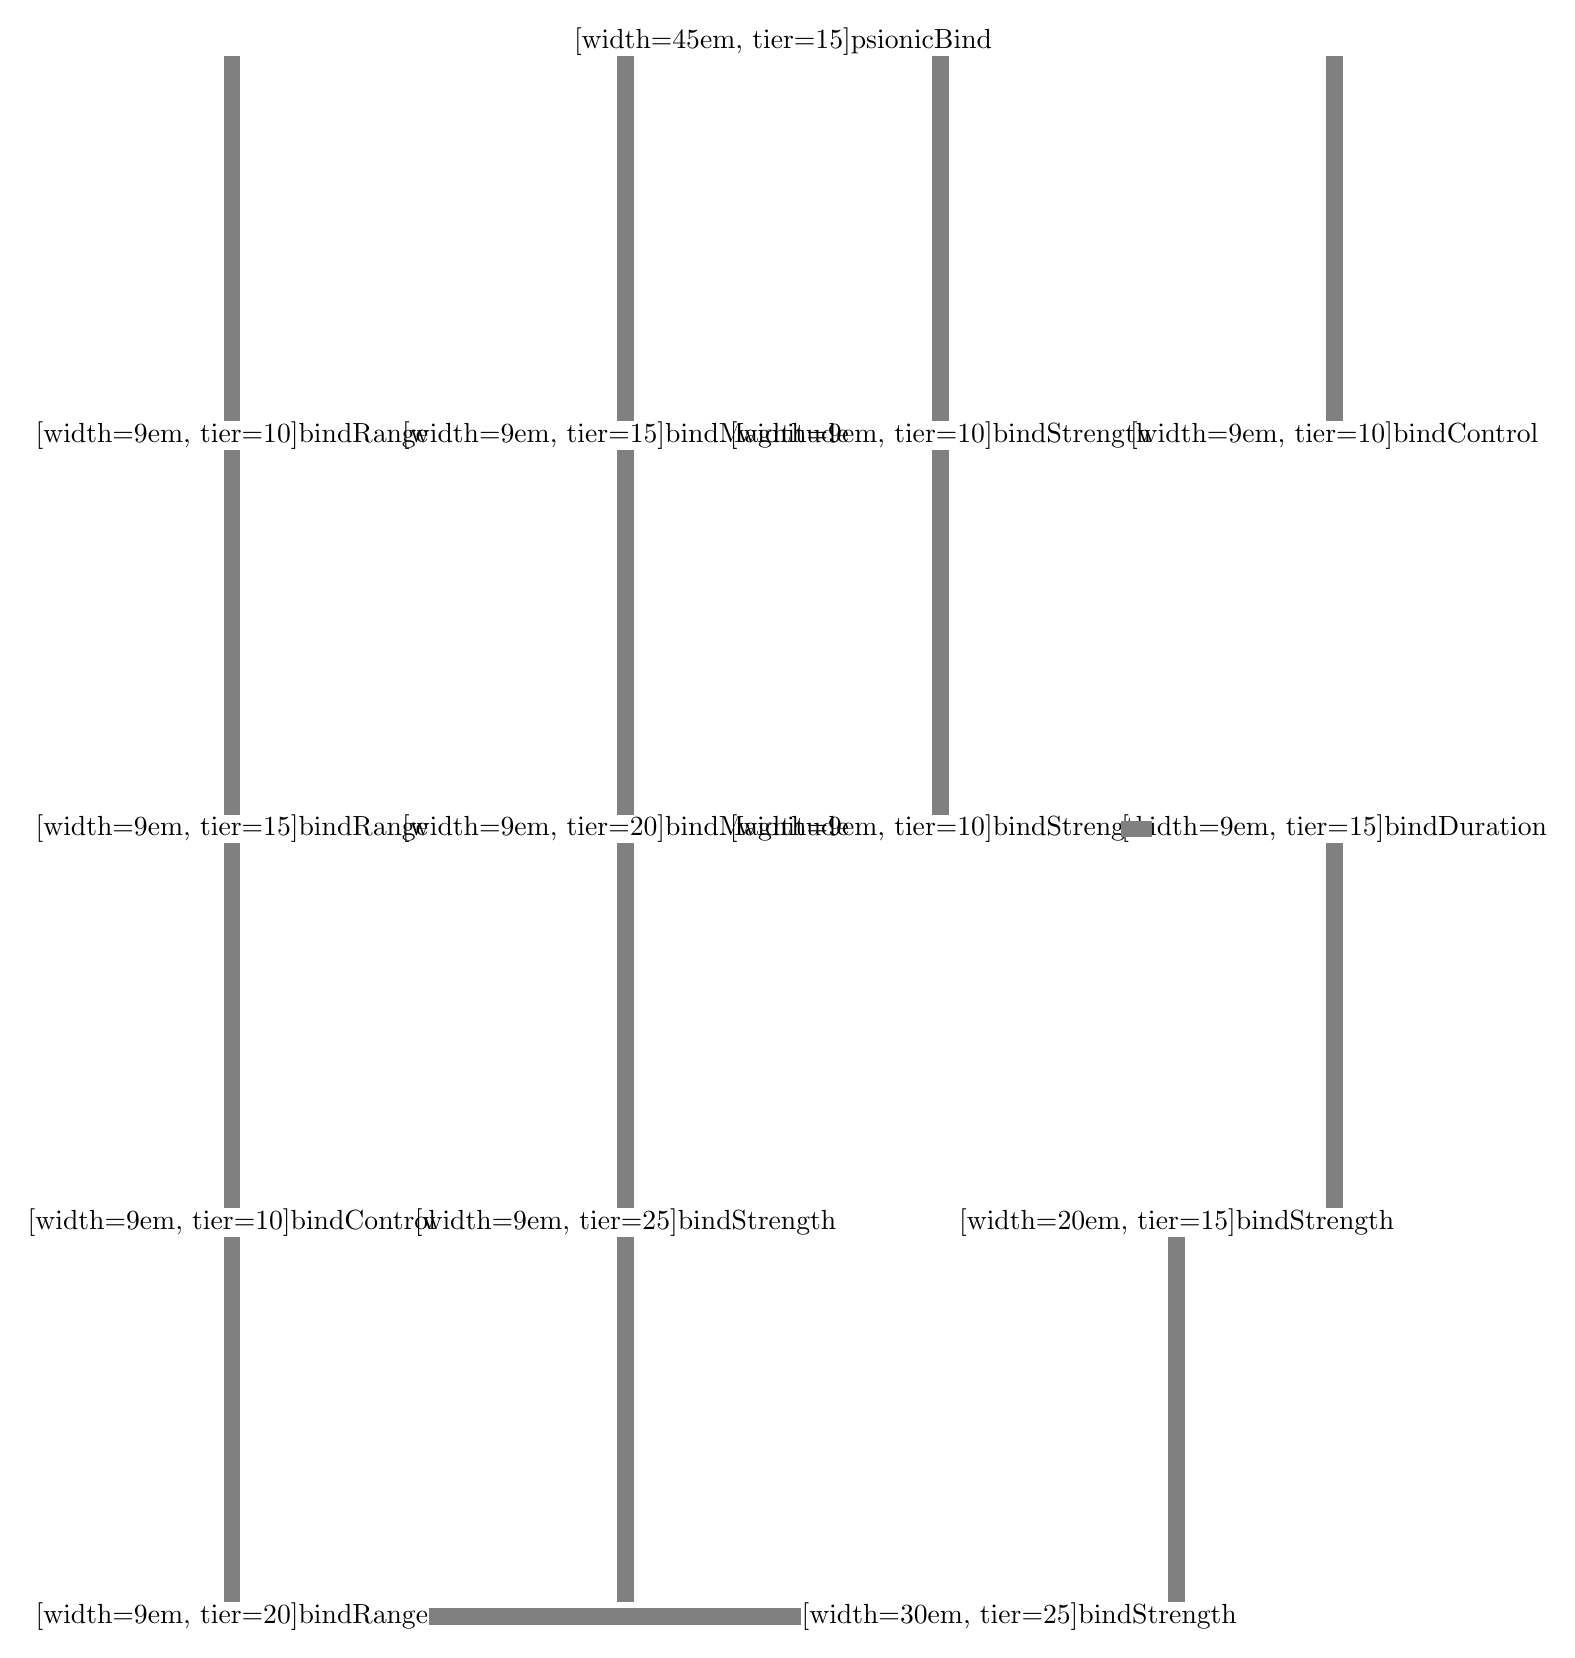
\begin{tikzpicture}
    \draw (-13,  -2) node(pr)[inner sep=0]{\TalentBox[width=45em, tier=15]{psionicBind}};
    \draw (-20,  -7) node(aa)[inner sep=0]{\TalentBox[width=9em,  tier=10]{bindRange}}
          (-15,  -7) node(ab)[inner sep=0]{\TalentBox[width=9em,  tier=15]{bindMagnitude}}
          (-11,  -7) node(ac)[inner sep=0]{\TalentBox[width=9em,  tier=10]{bindStrength}}
          ( -6,  -7) node(ad)[inner sep=0]{\TalentBox[width=9em,  tier=10]{bindControl}}
          (-20, -12) node(ba)[inner sep=0]{\TalentBox[width=9em,  tier=15]{bindRange}}
          (-15, -12) node(bb)[inner sep=0]{\TalentBox[width=9em,  tier=20]{bindMagnitude}}
          (-11, -12) node(bc)[inner sep=0]{\TalentBox[width=9em,  tier=10]{bindStrength}}
          ( -6, -12) node(bd)[inner sep=0]{\TalentBox[width=9em,  tier=15]{bindDuration}}
          (-20, -17) node(ca)[inner sep=0]{\TalentBox[width=9em,  tier=10]{bindControl}}
          (-15, -17) node(cb)[inner sep=0]{\TalentBox[width=9em,  tier=25]{bindStrength}}
          ( -8, -17) node(cd)[inner sep=0]{\TalentBox[width=20em, tier=15]{bindStrength}}
          (-20, -22) node(da)[inner sep=0]{\TalentBox[width=9em,  tier=20]{bindRange}}
          (-10, -22) node(db)[inner sep=0]{\TalentBox[width=30em, tier=25]{bindStrength}}
    ;

    \tikzstyle{bar}=[gray,-,>=stealth, line width=6pt]

    \draw [bar] (aa) -- (aa |- pr.south);
    \draw [bar] (ab) -- (ab |- pr.south);
    \draw [bar] (ac) -- (ac |- pr.south);
    \draw [bar] (ad) -- (ad |- pr.south);
    \draw [bar] (aa) edge (ba);
    \draw [bar] (ab) edge (bb);
    \draw [bar] (ac) edge (bc);
    \draw [bar] (bc) edge (bd);
    \draw [bar] (ba) edge (ca);
    \draw [bar] (bb) edge (cb);
    \draw [bar] (bd) -- (bd |- cd.north);
    \draw [bar] (ca) edge (da);
    \draw [bar] (da) edge (db);
    \draw [bar] (cb) -- (cb |- db.north);
    \draw [bar] (cd) -- (cd |- db.north);
\end{tikzpicture}
